% === RDTs
\section{Resonance Driving Terms}

Decapoles, due to their order, contribute to many RDTs. Indeed, 50 of them can be theoretically 
observed in simulations and measurements. In practice, the contributions of individual RDTs
become indistinguishable as many resonances overlap, making it impossible to isolate certain terms.
Up to a fixed order, some resonances, described in~\cref{appendix:rdts}, are unique to
certain multipoles. Those resonances, provided that they are sufficiently strong and close to the
beam, can be measured via their RDTs.

Of interest to the LHC Operation, is the RDT $f_{1004}$, driving the resonance $1Q_x - 4Q_y$.
It can be seen in the horizontal frequency spectrum at $-4Q_y$ with an amplitude dependence on
$J_y^2$. 
Figure~\cref{fig:decapoles:rdts:tune_diagram} shows a frequency
map~\cite{yannis_papaphilippou_detecting_nodate} of a simulation including decapolar field errors,
where their impact on the beam is easily noticeable. The \todo{red} particles evolving close to the
resonance are affected by it and are subject to large tune shifts. Eventually, those particles are 
lost when their amplitude becomes too large.

\begin{figure}[H]
    \centering
    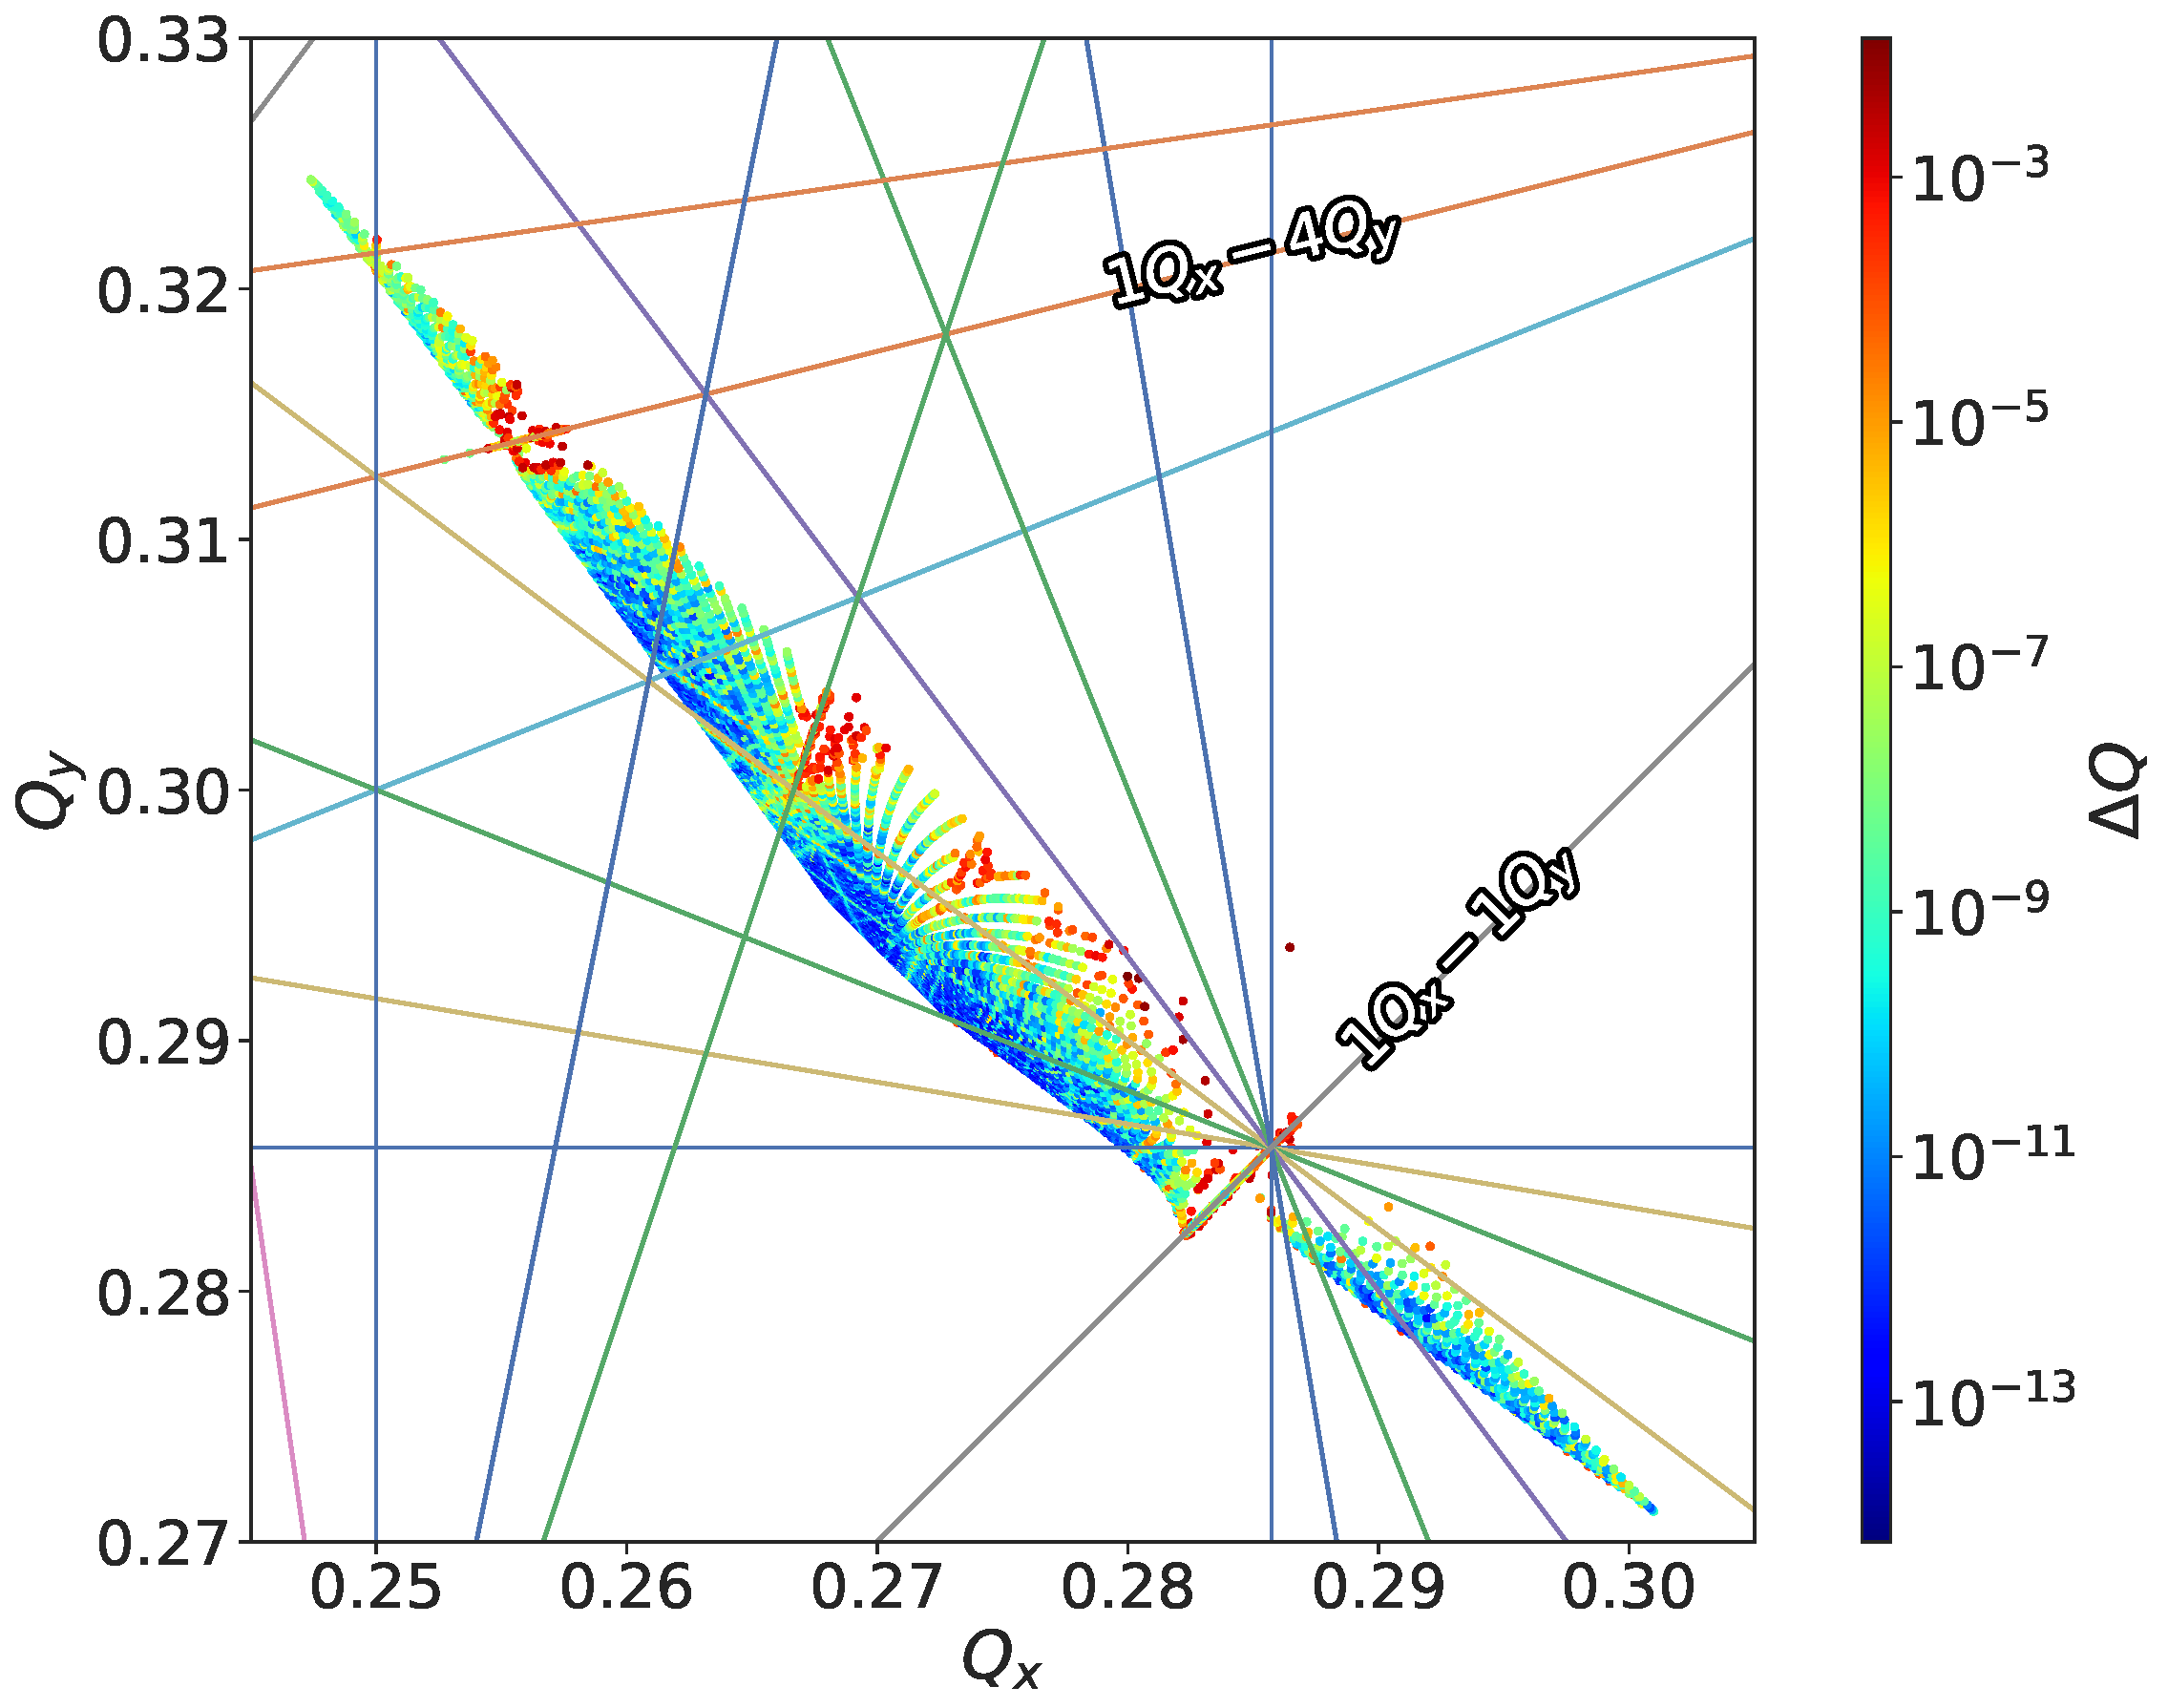
\includegraphics[width=0.8\textwidth]{./images/tune_diagram_f1004.pdf}
    \caption{Frequency map at injection energy, with decapolar field errors and nominal settings for
    landau octupoles. The highlighted resonance (1,-4), excited by decapoles, shows a degradation
    over 20,000 turns. The tune shift between the start and the end of the simulation is indicated
    in colour. \todo{change colormap}}
    \label{fig:decapoles:rdts:tune_diagram}
\end{figure}

Measuring turn-by-turn data without using any excitation is not a viable option as amplitudes are
not large enough. Spectral lines are indeed usually impossible to discern from the noise floor, 
making RDTs not measurable.
Measurements are hence taken with an AC-Dipole, introducing quadrupolar-like field errors in the 
linear regime~\cite{carlier_nonlinear_2020} and more complex effects in the non linear regime.
In practice, those effects are neglected. \textit{Forced} RDTs are measured with an
AC-Dipole and treated as \textit{free} as no compensation is applied.

Such forced measurements were taken for the first time in the LHC to observe the $f_{1004}$ RDT
at injection energy. The frequency line of the resonance $1Q_x - 4Q_y$ is seen at $4Q_y$ in the
horizontal spectrum, as shows \cref{fig:decapoles:rdts:spectrum_f1004}.

\begin{figure}[H]
    \centering
    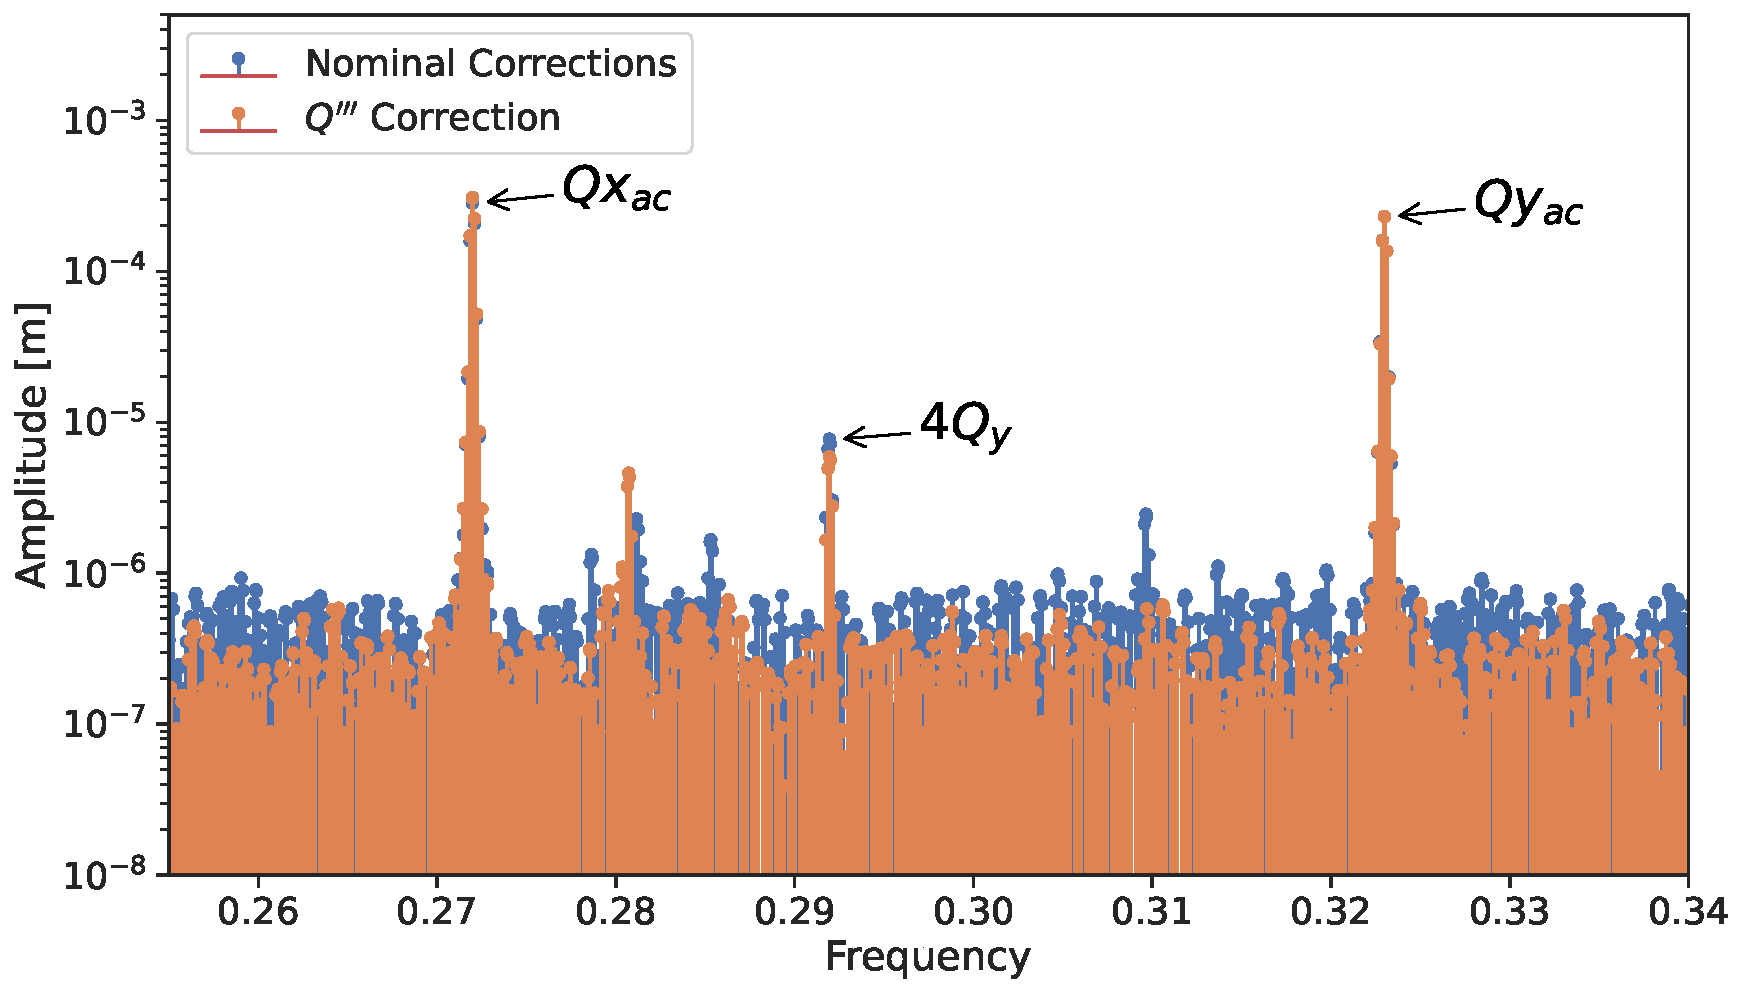
\includegraphics[width=0.9\textwidth]{./images/f1004x_spectrum.pdf}
    \caption{Horizontal frequency spectrum of turn-by-turn data, with nominal and beam-based
    corrections for the third order chromaticity $Q'''$. The $1Q_x - 4Q_y$ resonance can be seen
    at $-4Q_y$ with different amplitudes for each correction scheme.}
    \label{fig:decapoles:rdts:spectrum_f1004}
\end{figure}

Moreover, \cref{fig:decapoles:rdts:spectrum_f1004} shows that the amplitude of this resonance line
decreases upon application of beam-based corrections for $Q'''$. This translates to the amplitude
of the RDT $f_{1004}$, as seen in \cref{fig:decapoles:rdts:f1004_dq3}.

\begin{figure}[H]
    \centering
    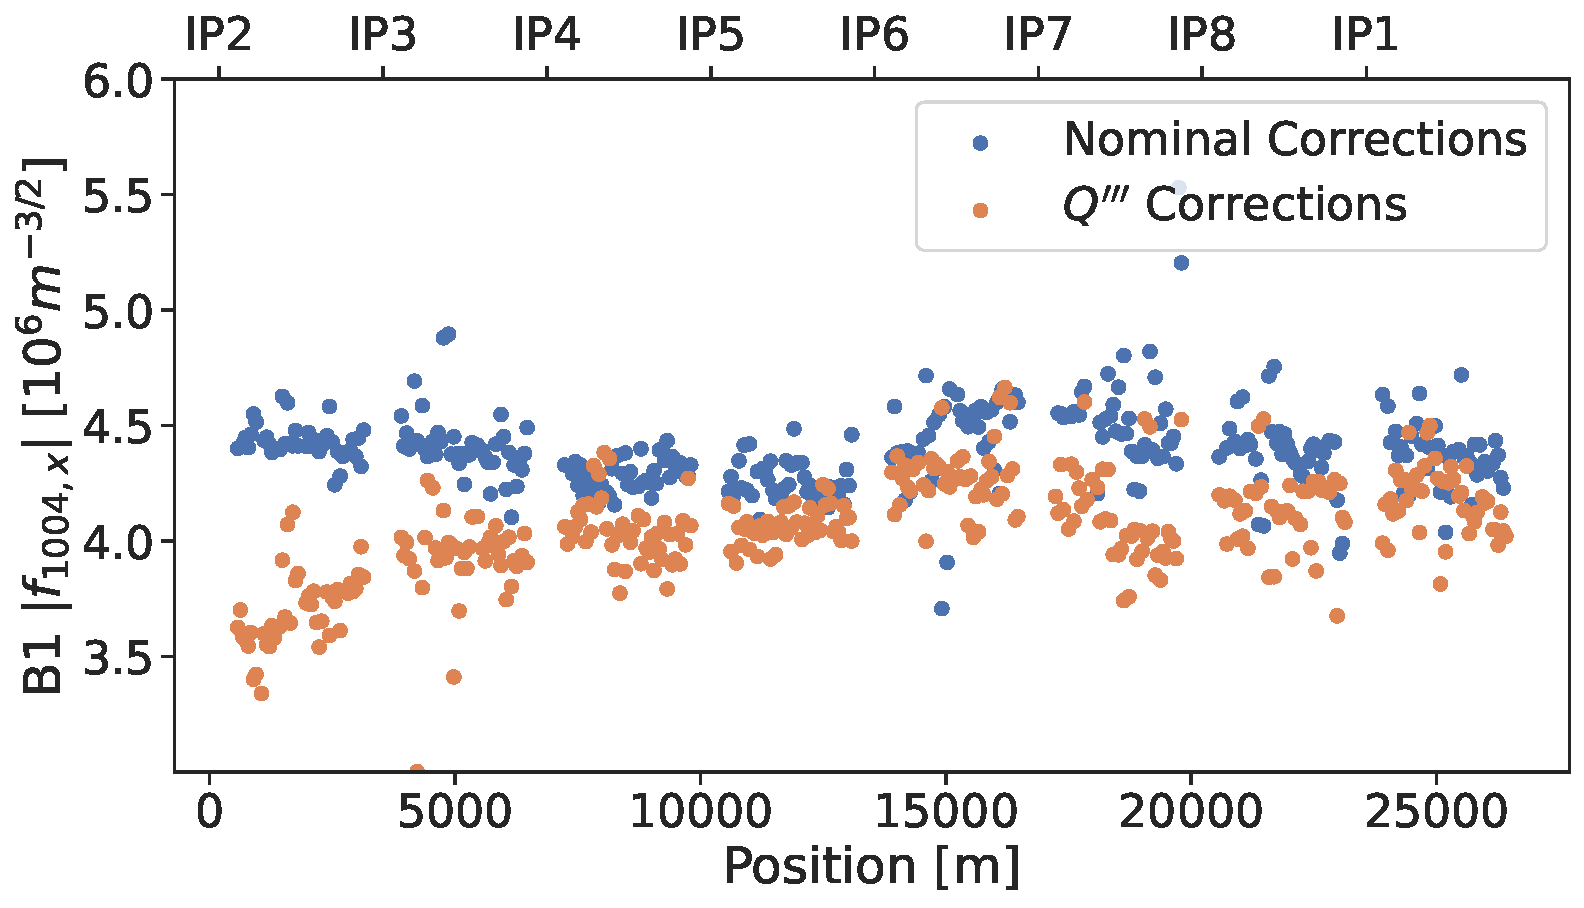
\includegraphics[width=0.9\textwidth]{./images/f1004_dq3.pdf}
    \caption{Amplitude of the RDT $f_{1004}$ generated by normal decapoles, measured before and
    after having applied beam-based corrections of the third order chromaticity $Q'''$.}
    \label{fig:decapoles:rdts:f1004_dq3}
\end{figure}


\todo{
    Measurements: \\
    \begin{itemize}
        \item 2022 Q'' and Q''' corrections 2022-04-24
        \item 2022-10-19 Virgin machine
        \item 2023-easter (FiDeL)
        \item 2023-06-14 MD9549 (FiDeL and Q'''/ RDT corr)
    \end{itemize}
    Effect of RCO correction on RDT f1004 \\
    Response
}

% ---------------------------------------
%         Decapole Contribution
% ---------------------------------------
\subsection{\todo{Decapolar Contribution}}


% ---------------------------------------
%        Higher Order Contribution
% ---------------------------------------
\subsection{\review{Higher Order Contributions}}

% Measurements in 
% /afs/cern.ch/work/m/mlegarr2/public/beta_beat_output/2024-05-21

To produce collisions at top energy, \textit{crossing angles} are introduced via the orbit
correctors located in the triplets, before the separation dipoles and the matching section of the
interaction regions (\texttt{MCBX}, \texttt{MCBY} and \texttt{MCBC})~\cite{de_maria_lhc_2008}. Those
collisions happen with a small $\beta*$, currently 30cm, requiring strong quadrupolar fields from
the triplets.

At such $\beta$, those triplets also generate strong dodecapolar field errors. Because of the
crossing-angles, feed-down appears and lower-order fields can be observed.
Such feed-down to decapolar fields was observed during the first commissioning of Run~3, in
2022~\cite{maclean_prospects_2022}.
\cref{fig:decapoles:f1004_from_feeddown} shows how the RDT $f_{1004}$, normally affected by
decapoles, varies with the application of crossing angles.

\begin{figure}[H]
    \centering
    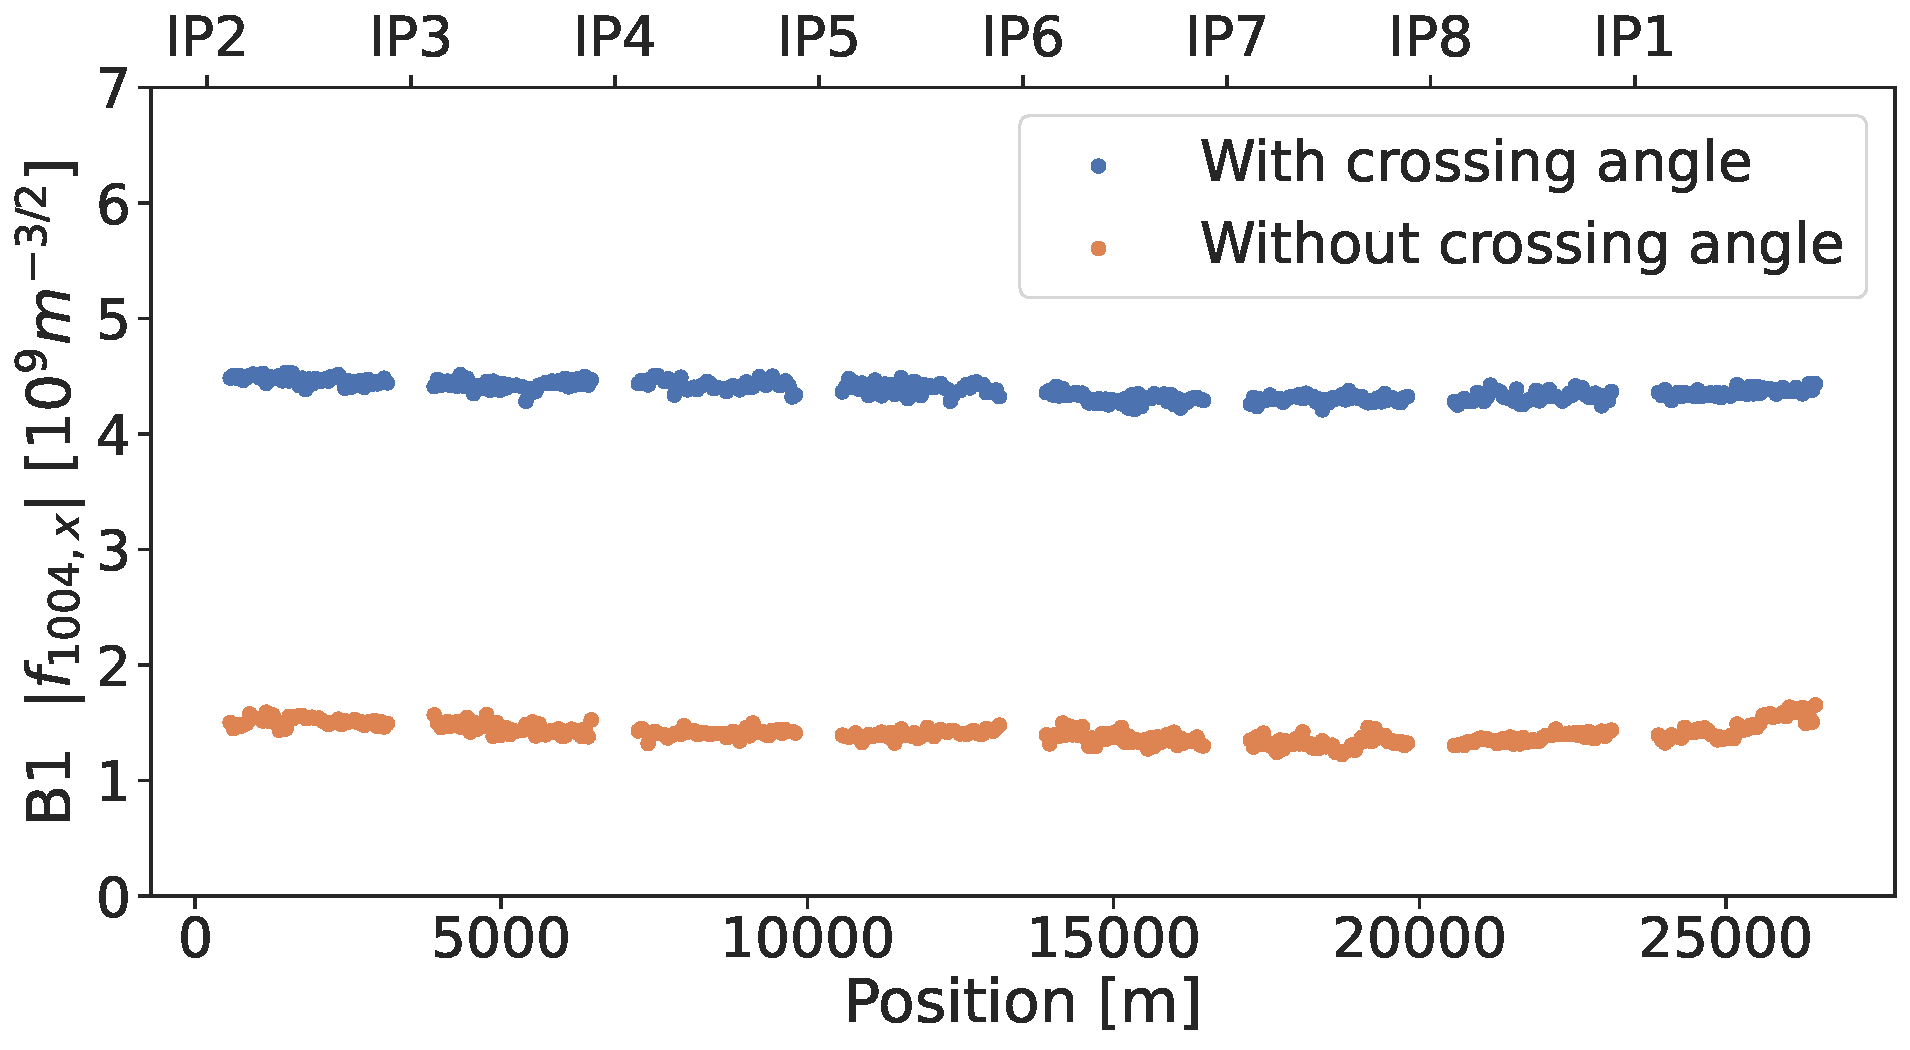
\includegraphics[width=0.9\textwidth]{./images/f1004x_feed-down_b6_triplets.pdf}
    \caption{}
    \label{fig:decapoles:f1004_from_feeddown}
\end{figure}

Such a contribution is though not expected at injection energy, as the triplets aren't powered as
much as at top energy, $\beta*$ being set at around $10$m. Moreover, not crossing angle

% ---------------------------------------
%        Lower Order Contribution
% ---------------------------------------
\subsection{\todo{Lower Order Contributions}}

% http://localhost:8888/lab/workspaces/auto-d/tree/work_afs2/jupyter/resonance_driving_terms/measurements/2024-03-13_b3_b4_effect_on_b5/Sextupoles_and_Octupoles.ipynb

% ------- Introduction
\subsubsection{\review{First Observation}}

As described in \cref{appendix:transfer_maps}, multipoles can combine to create fields that are seen
as higher orders when considering higher orders of the BCH expansion.
For decapoles, combinations of several sextupoles and sextupoles with octupoles give rise to
decapolar-like fields, as described in
\cref{table:appendix:transfer_maps:bch_resulting_orders_combination}. The following parts of this
section will describe those combinations.

This effect was observed in 2022 during Run 3's commissioning. Routine corrections of the non-linear
chromaticity $Q''$ and $Q'''$ were performed, and RDT measurements taken before and after their
correction. As $Q'''$ was corrected, the expectation was that the RDT $f_{1004}$ would also lower
with the reduction of the decapolar strengths $K_5$. However, an increase of the RDT was observed,
as shows \cref{fig:decapoles:f1004_dq2_dq3}.

\begin{figure}[H]
    \centering
    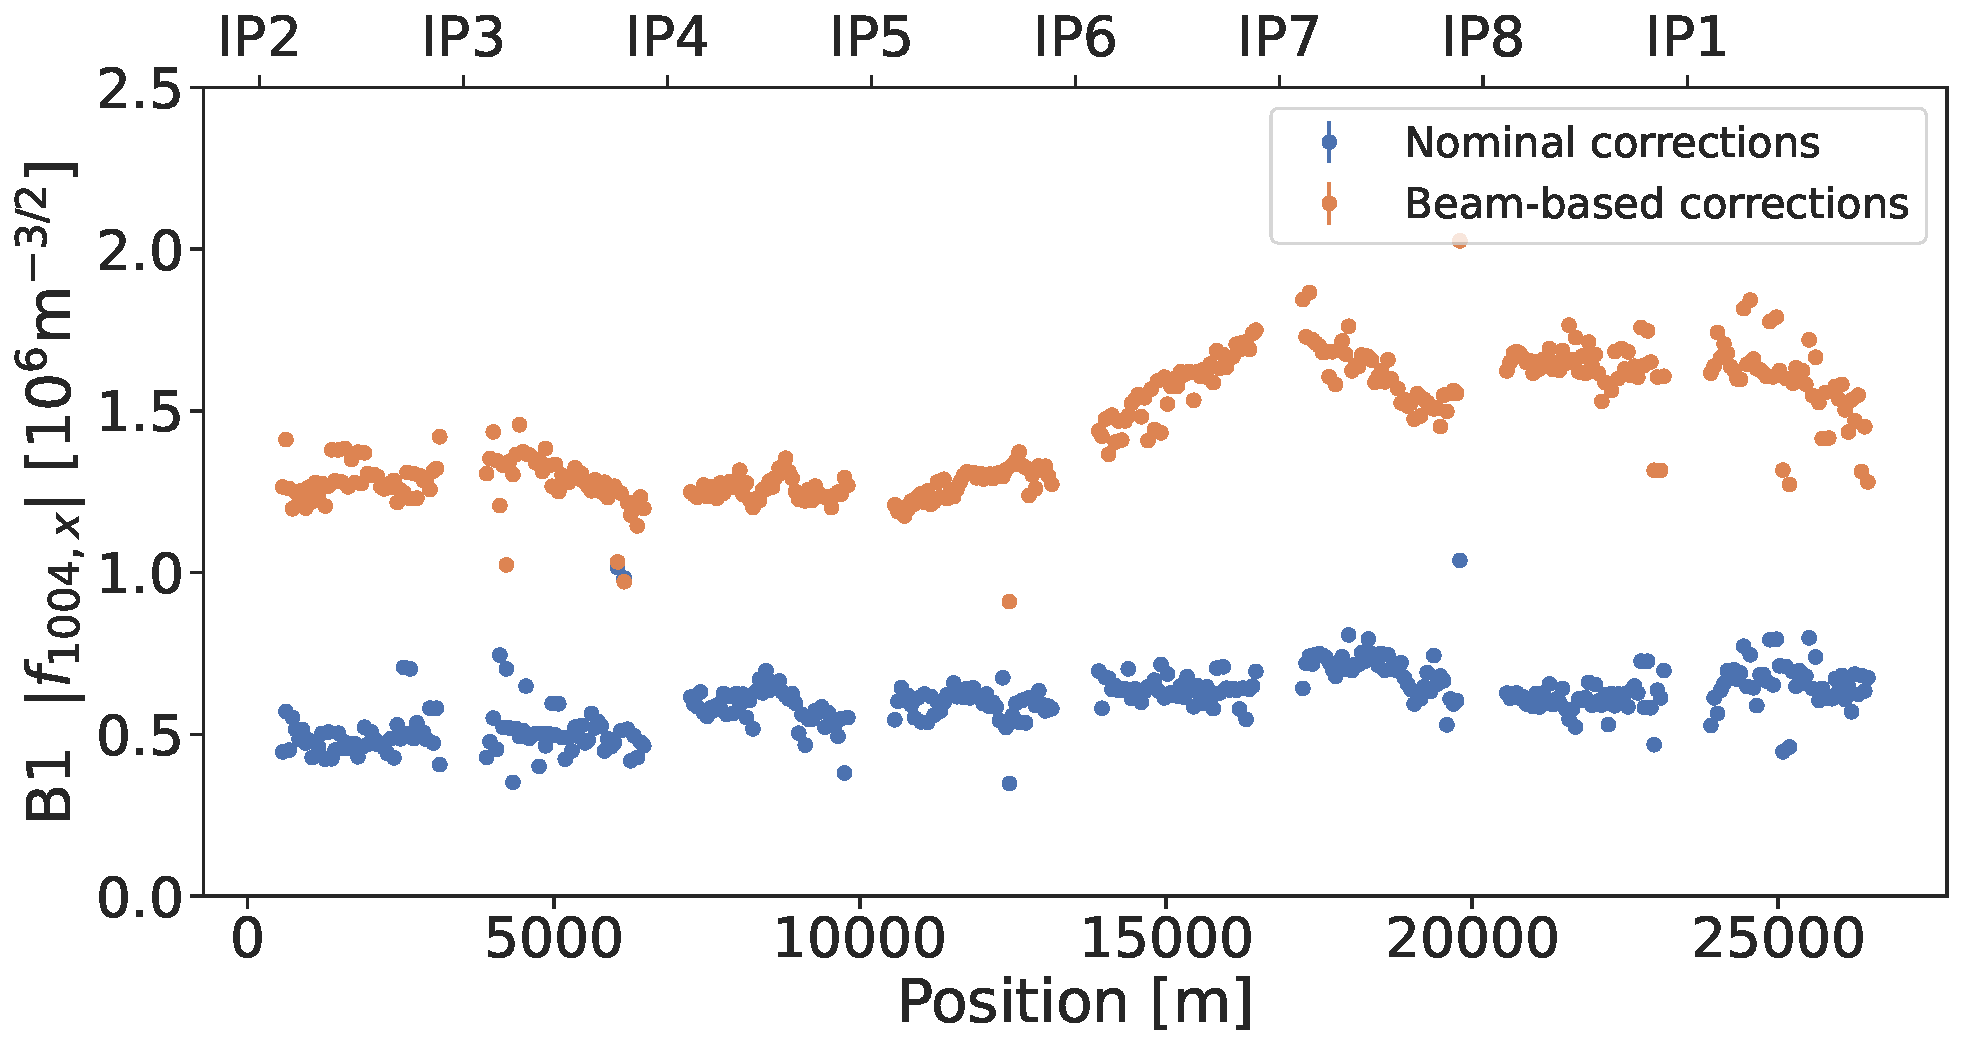
\includegraphics[width=0.9\textwidth]{./images/f1004_dq2_dq3_2022.pdf}    
    \caption{Non intuitive increase of the RDT $f_{1004}$ after application of the $Q''$ and $Q'''$
    corrections.\todo{redo plot}}
    \label{fig:decapoles:f1004_dq2_dq3}
\end{figure}


% ------- Action dependance
\subsubsection{\review{Action Dependance and Analysis}}

Resonance lines in the frequency spectrum are often contributed to by several multipoles. Some lines
start getting a contribution with rather high multipole orders, like the RDT $f_{1004}$ considered
here. The line $4Q_y$ in the horizontal spectrum is indeed contributed to by decapoles and then only
by decatetrapoles. When the main contributing field alone is varied, it is easy to reconstruct the
RDT, as its fit is only dependant its action dependance ($\propto J_x^{*} J_y^{*}$). Several
turn-by-turn measurements at the same configuration can be taken wit varying kick amplitudes,
refining the RDT value with more data points for the fit.

Considering the contribution of lower order multipoles is a bit trickier, as the second order RDTs
change the dependance of the frequency line~\cite{franchi_first_2014}. In order to be able to
extract the RDT from several turn by turn measurements, the same kick amplitude must then be used.

%\todo{simulation plot of varying amplitudes for Q' = 2 and noise created from it}

% ------- Sextupoles
\subsubsection{\todo{Sextupoles}}

At the third order of the BCH expansion, the combination of two sextupoles yields a decapolar-like
expression. Derivation of such a combination can be found in
\cref{appendix:transfer_map:two_sextupoles}. The resulting Hamiltonian indeed is similar to
the terms of a decapole, dropping the $p_{x,y}$ terms for readability:

\begin{equation}
    \begin{aligned}
         (H_3)^3 &\propto \frac{1}{48} \left(x^5 - 2x^3y^2 - 3xy^4 \right)\\
                 &\sim    x^5 - 10x^3y^2 + 5xy^4.
    \end{aligned}
\end{equation}

This means that, during normal operation of the machine, decapolar observables will be altered when
adjusting parameters such as the linear chromaticity $Q'$. A simulation was run with injection
optics and varying the linear chromaticity $Q'$. The resulting effect on the RDT $f_{1004}$ can be
seen in \cref{decapoles:rdts:simulated_f1004_from_sextupoles}.

\begin{figure}[H]
    \centering
    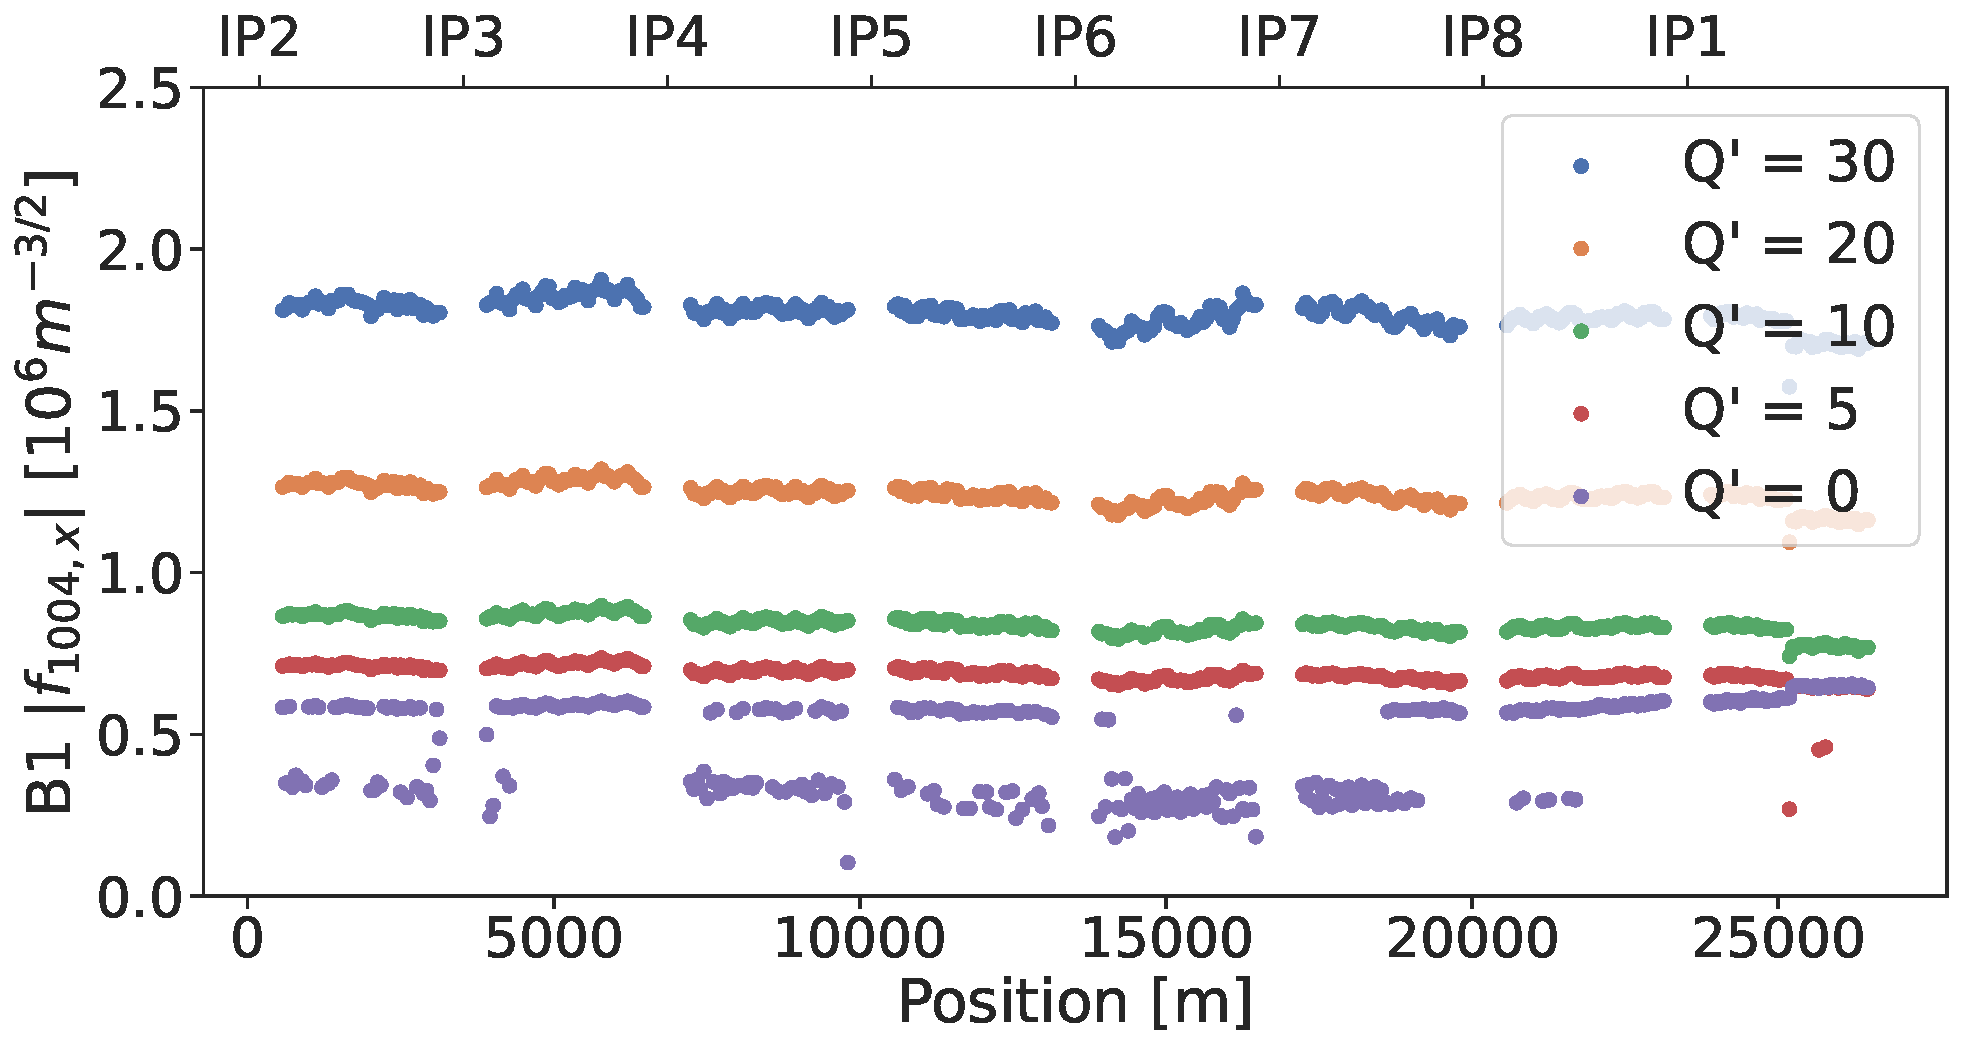
\includegraphics[width=0.9\textwidth]{./images/f1004/f1004_dq.pdf}
    \caption{Simulated change of the decapolar RDT $f_{1004}$ depending of the desired linear
    chromaticity $Q'$ generated by sextupoles.}
    \label{decapoles:rdts:simulated_f1004_from_sextupoles}
\end{figure}



\cref{decapoles:rdts:measured_f1004_from_sextupoles} shows measurements done with varying values
for $Q'$. 

\begin{figure}[H]
    \centering
    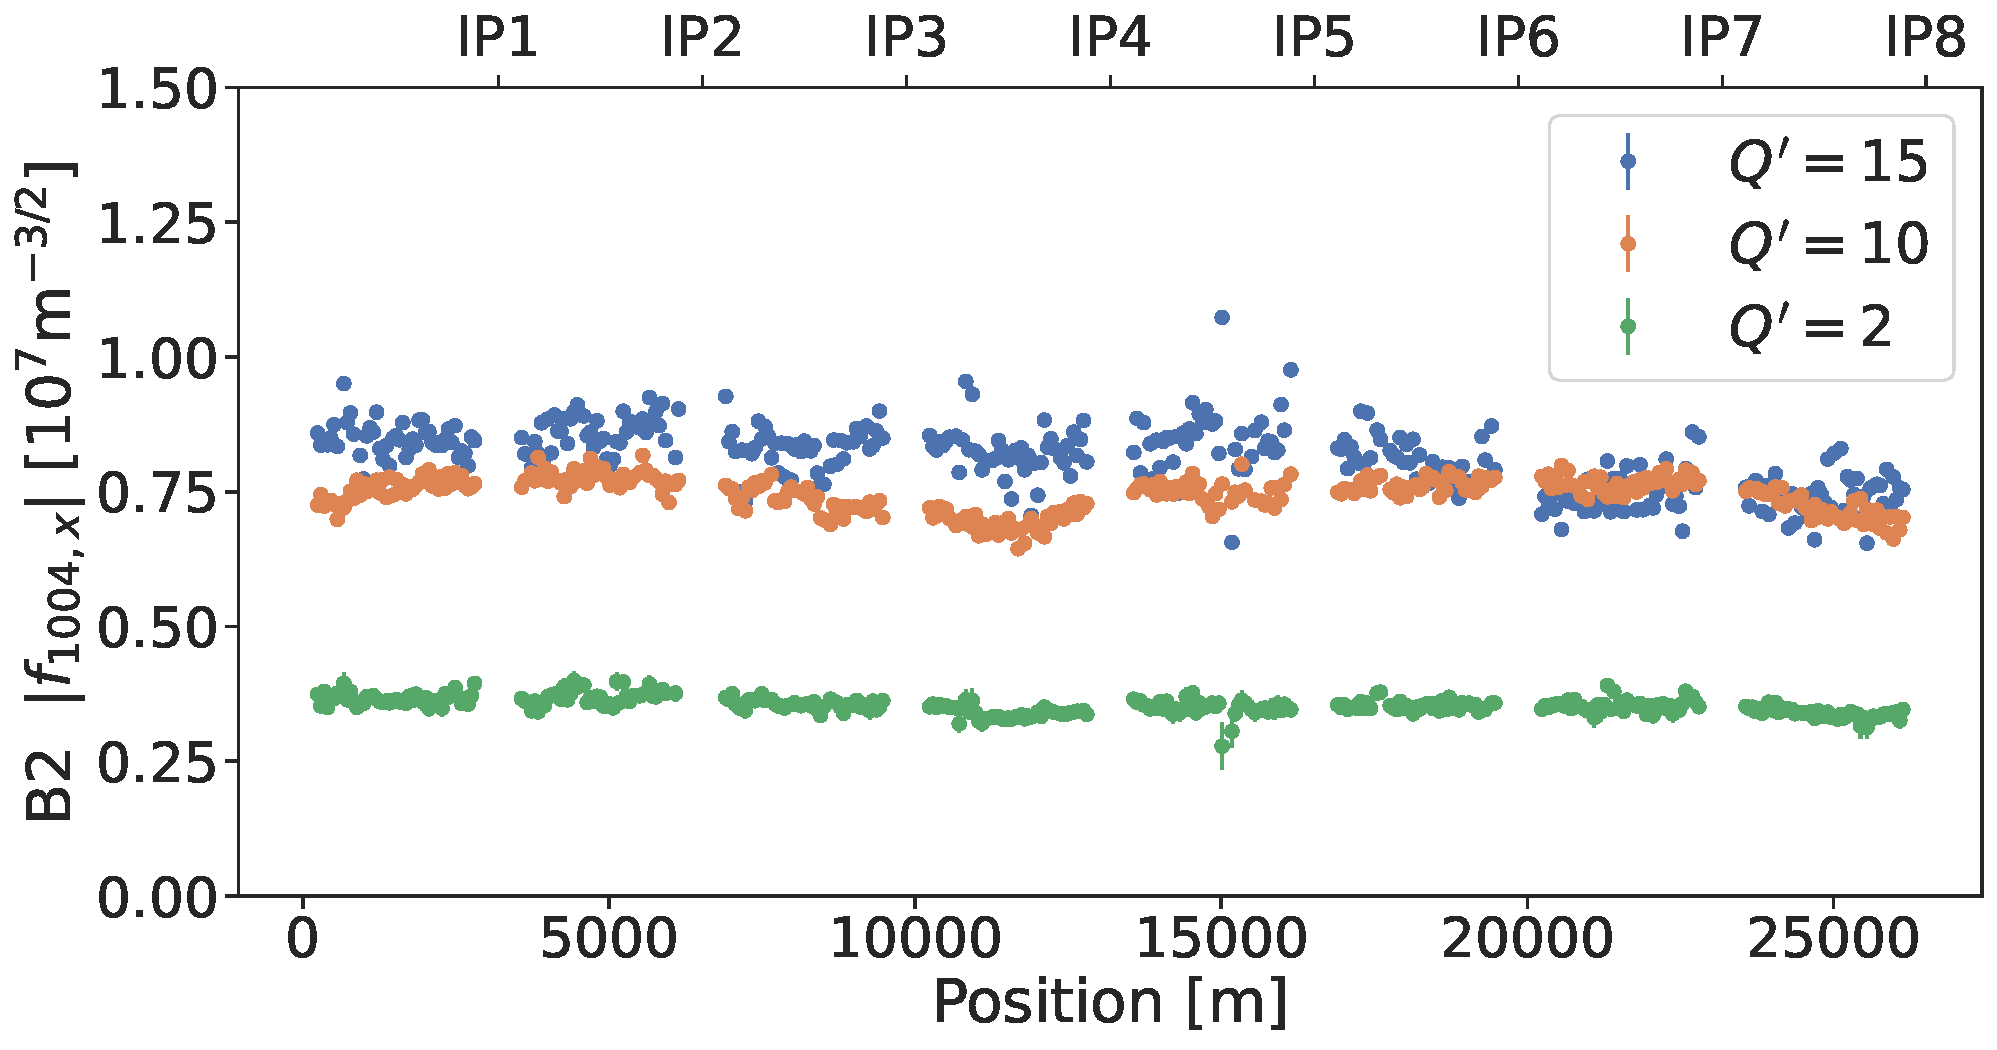
\includegraphics[width=0.9\textwidth]{./images/f1004/f1004x_q2_q10_q15.pdf}
    \caption{Measured change of the decapolar RDT $f_{1004}$ depending of the desired linear
    chromaticity $Q'$ generated by sextupoles.}
    \label{decapoles:rdts:measured_f1004_from_sextupoles}
\end{figure}

%Measurements are typically performed at $Q' = 3$

% ------- Sextupole + Octupole
\subsubsection{\todo{Sextupoles and Octupoles}}

\begin{figure}[H]
    \centering
    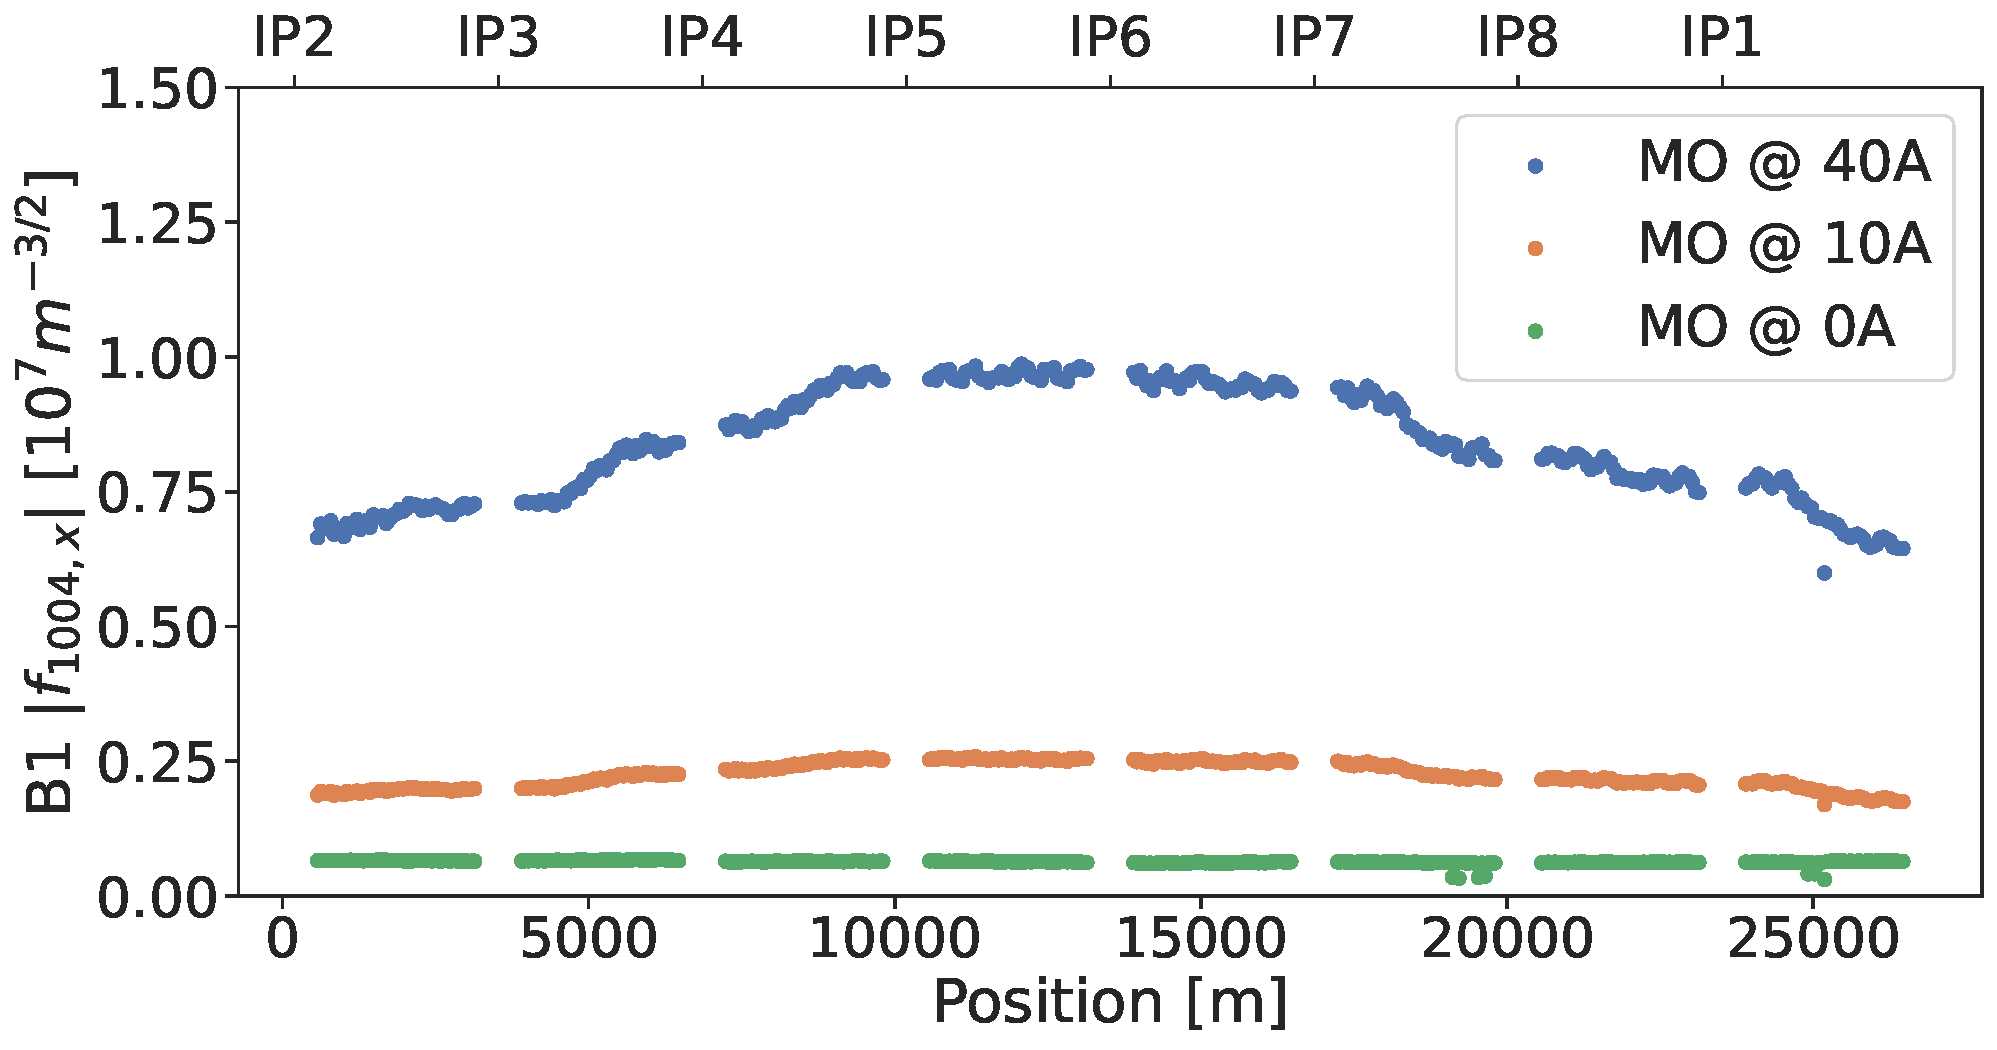
\includegraphics[width=0.9\textwidth]{./images/f1004/f1004_mo.pdf}
    \caption{Simulated change of the decapolar RDT $f_{1004}$ depending of the landau octupoles 
    (\texttt{MO}) strength.}
    \label{}
\end{figure}

\begin{figure}[H]
    \centering
    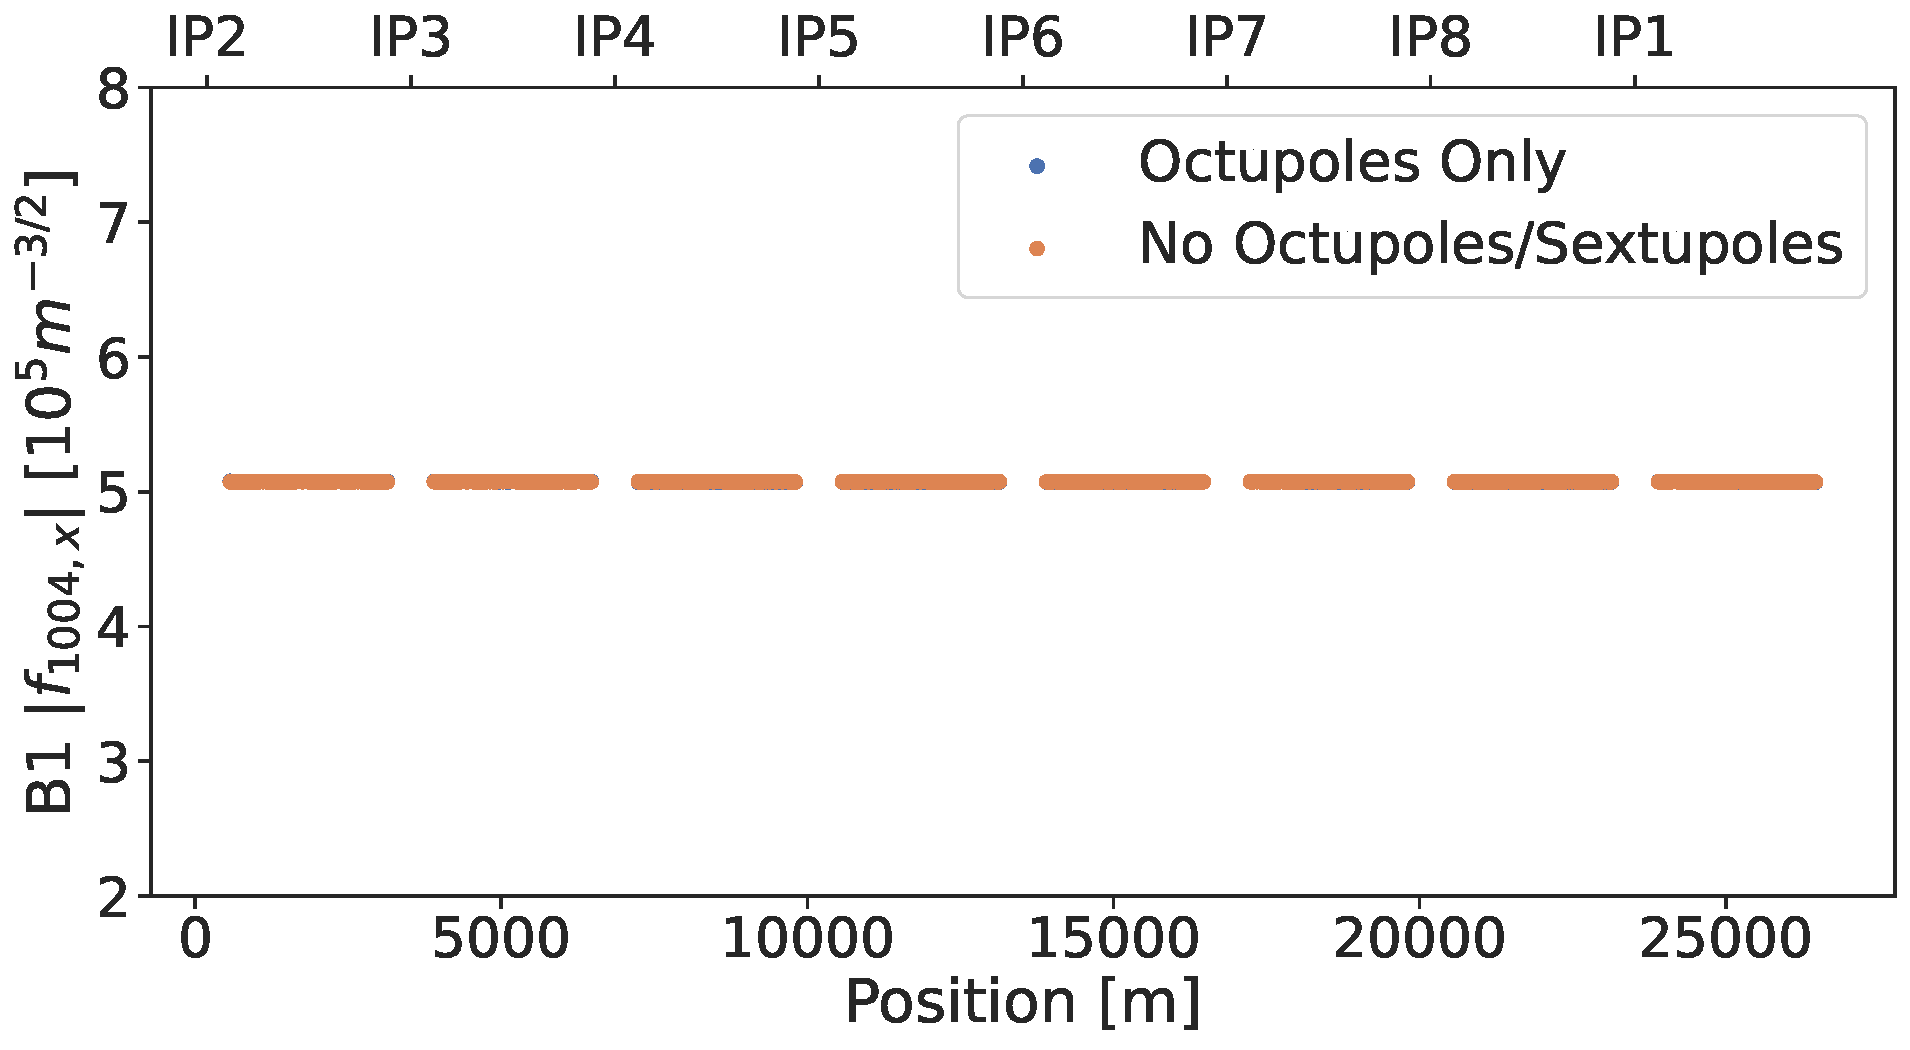
\includegraphics[width=0.9\textwidth]{./images/f1004/f1004_no_ms.pdf}
    \caption{Simulated decapolar RDT $f_{1004}$ with two different schemes. First scheme has
    lattice sextupoles turned off and octupoles turned on. Second scheme has all sextupoles of the
    lattice turned off and octupoles turned off as well. No difference is seen, as expected from
    the equations.}
    \label{}
\end{figure}

\begin{figure}[H]
    \centering
    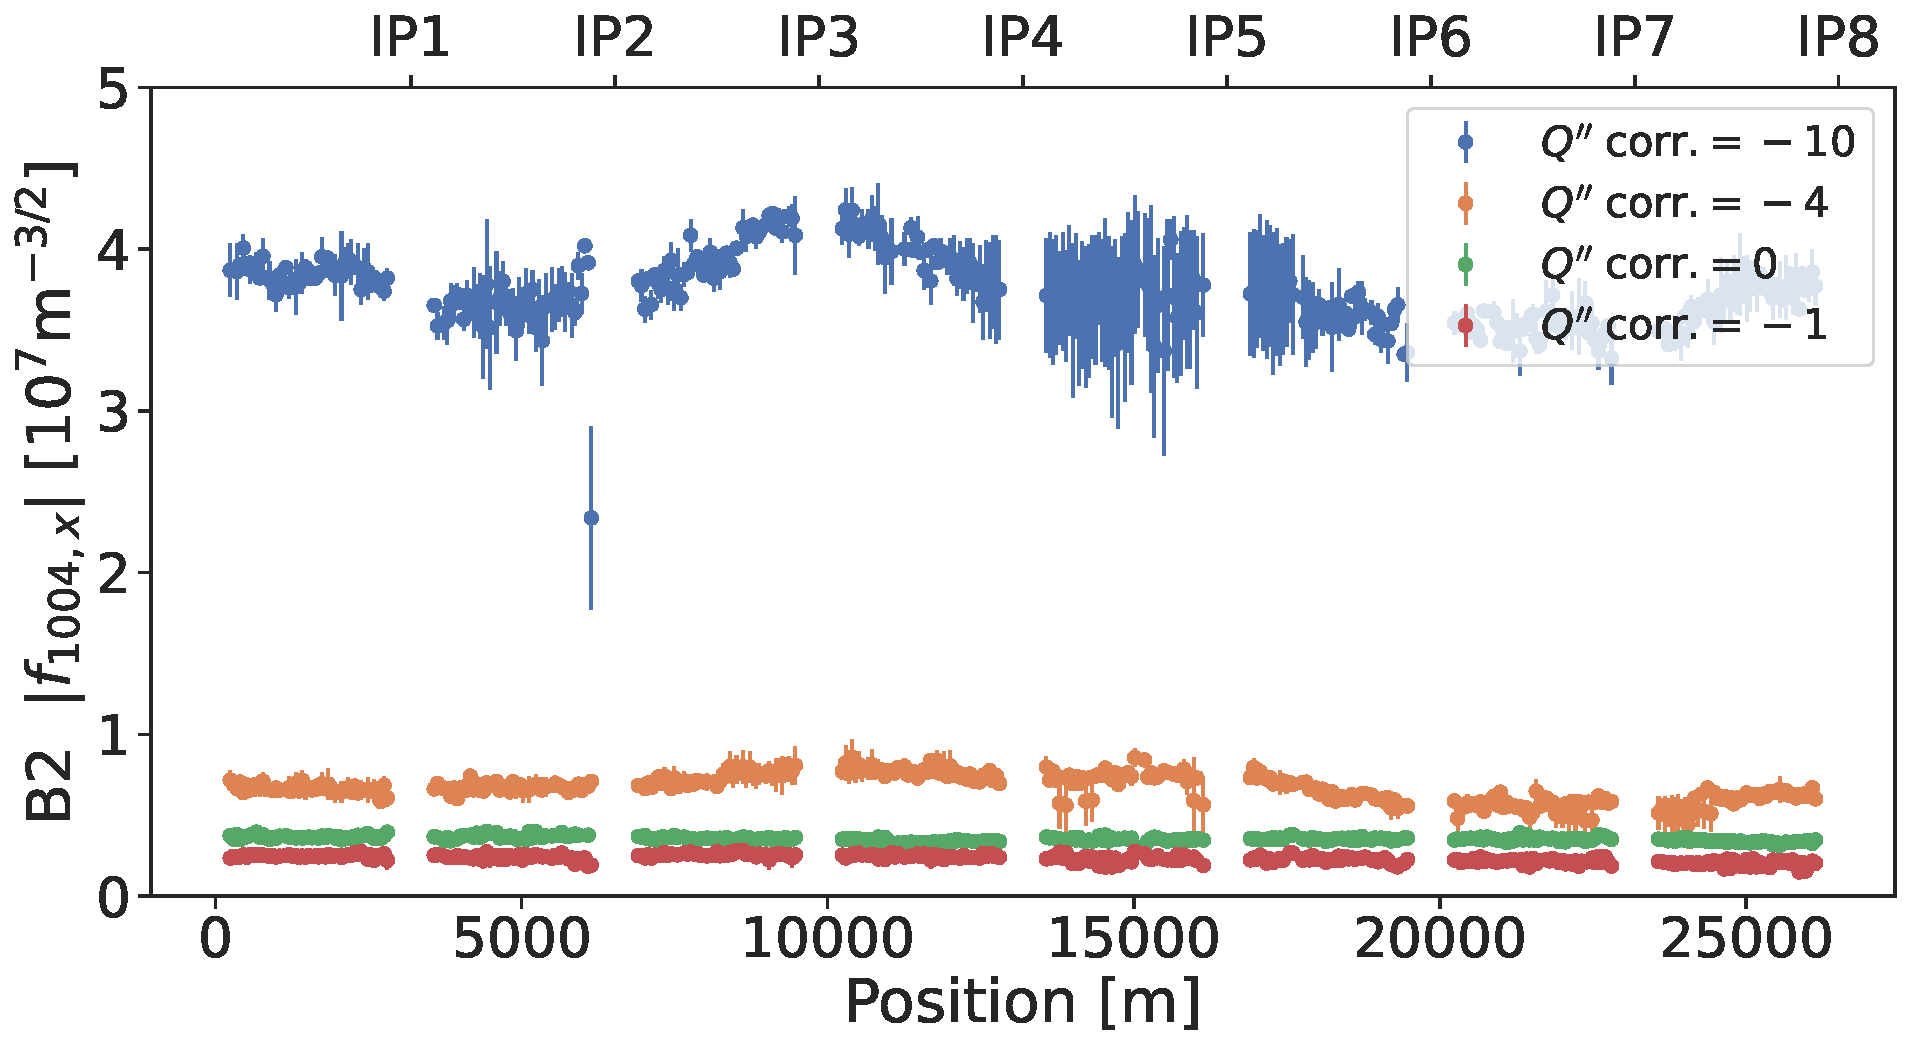
\includegraphics[width=0.9\textwidth]{./images/f1004/f1004x_mco_corr.pdf}
    \caption{Different MCO Corr.}
    \label{decapoles:rdts:measured_f1004_mco}
\end{figure}